% ================= CHAPTER 4 =================
\chapter{Experimental Results and Deployment}
\vspace{0.5cm}
\minitoc
\vspace{1cm}

% ── Introduction (unnumbered) ────────────────────────────────────────────────
\section*{Introduction}
\addcontentsline{toc}{section}{Introduction}

This chapter presents and discusses the experimental results obtained by applying the methodology described in Chapter 3. We begin by describing the software environment used for development. We then report the classification performance of all six trained models, the results of the statistical validation (Bootstrap CI and ANOVA), the XAI analysis (SHAP, LIME, PFI triangular validation for ML models and GradientExplainer/LIME for DL models), and the adversarial robustness evaluation (FGSM and PGD). We also compare our results against the state-of-the-art works reviewed in Chapter 2. Finally, we justify the selection of LightGBM as the deployed model and describe the architecture and features of the production web application.

% ── 4.1 Software Environment ─────────────────────────────────────────────────
\section{Software Environment}

\subsection{Development Environments}

\paragraph{Google Colab.}
All model training, evaluation, and XAI experiments were conducted in Google Colaboratory, a cloud-hosted Jupyter notebook environment provided by Google. Colab offers free GPU access (NVIDIA T4 or A100 depending on availability) and 12.7 GB of RAM, which is sufficient for training the six models on the 101,063-URL PhishFOE dataset. Its integrated support for Python scientific libraries (NumPy, pandas, scikit-learn, TensorFlow, LightGBM, SHAP, LIME) made it the ideal environment for rapid experimentation.

\paragraph{Visual Studio Code.}
The FastAPI backend and Next.js frontend were developed in Visual Studio Code (VS Code), Microsoft's lightweight open-source code editor. VS Code's built-in Git integration, Python and JavaScript extensions, IntelliSense autocomplete, and integrated terminal streamlined the development and debugging workflow for the deployed application.

\subsection{Frameworks and Technologies}

Figure~\ref{fig:frameworks} presents the logos of the main technologies used in this project.

\begin{figure}[H]
\centering
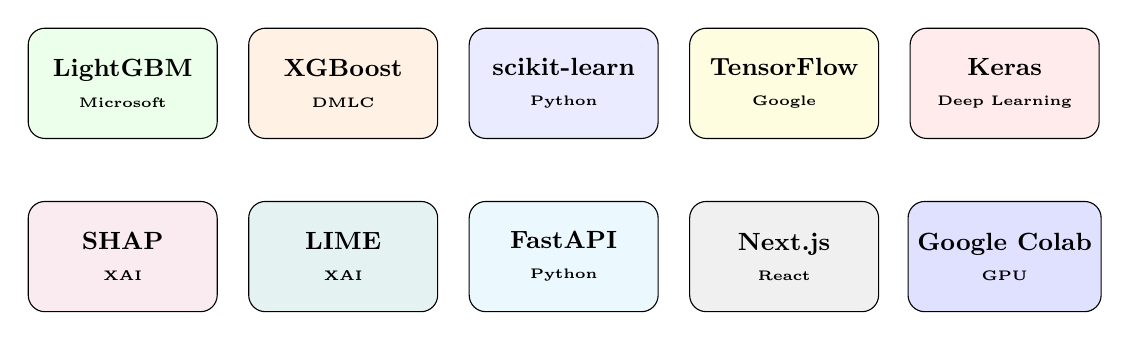
\begin{tikzpicture}
    % Row 1 — ML/DL
    \node[draw, rounded corners=6pt, fill=green!8,  minimum width=2.4cm, minimum height=1.4cm, align=center, font=\small\bfseries] at (0,    0) {LightGBM\\{\tiny Microsoft}};
    \node[draw, rounded corners=6pt, fill=orange!10, minimum width=2.4cm, minimum height=1.4cm, align=center, font=\small\bfseries] at (2.8,  0) {XGBoost\\{\tiny DMLC}};
    \node[draw, rounded corners=6pt, fill=blue!8,   minimum width=2.4cm, minimum height=1.4cm, align=center, font=\small\bfseries] at (5.6,  0) {scikit-learn\\{\tiny Python}};
    \node[draw, rounded corners=6pt, fill=yellow!12,minimum width=2.4cm, minimum height=1.4cm, align=center, font=\small\bfseries] at (8.4,  0) {TensorFlow\\{\tiny Google}};
    \node[draw, rounded corners=6pt, fill=red!8,    minimum width=2.4cm, minimum height=1.4cm, align=center, font=\small\bfseries] at (11.2, 0) {Keras\\{\tiny Deep Learning}};
    % Row 2 — XAI / Deployment
    \node[draw, rounded corners=6pt, fill=purple!8, minimum width=2.4cm, minimum height=1.4cm, align=center, font=\small\bfseries] at (0,   -2.2) {SHAP\\{\tiny XAI}};
    \node[draw, rounded corners=6pt, fill=teal!10,  minimum width=2.4cm, minimum height=1.4cm, align=center, font=\small\bfseries] at (2.8, -2.2) {LIME\\{\tiny XAI}};
    \node[draw, rounded corners=6pt, fill=cyan!8,   minimum width=2.4cm, minimum height=1.4cm, align=center, font=\small\bfseries] at (5.6, -2.2) {FastAPI\\{\tiny Python}};
    \node[draw, rounded corners=6pt, fill=gray!12,  minimum width=2.4cm, minimum height=1.4cm, align=center, font=\small\bfseries] at (8.4, -2.2) {Next.js\\{\tiny React}};
    \node[draw, rounded corners=6pt, fill=blue!12,  minimum width=2.4cm, minimum height=1.4cm, align=center, font=\small\bfseries] at (11.2,-2.2) {Google Colab\\{\tiny GPU}};
\end{tikzpicture}
\caption{Main frameworks and technologies used in the PhishShield project. Top row: machine learning and deep learning libraries. Bottom row: XAI tools, API framework, web frontend, and cloud computing environment.}
\label{fig:frameworks}
\end{figure}

\begin{itemize}
    \item \textbf{LightGBM / XGBoost / scikit-learn:} Python libraries for gradient boosting and classical ML model training, evaluation, and feature importance.
    \item \textbf{TensorFlow / Keras:} Deep learning framework for building and training the MLP, CNN, and LSTM architectures with GPU acceleration.
    \item \textbf{SHAP:} Open-source library providing TreeExplainer (ML) and GradientExplainer (DL) for exact and approximate Shapley value computation.
    \item \textbf{LIME:} Model-agnostic local explanation library applied to all six models via a \texttt{predict\_proba} wrapper.
    \item \textbf{FastAPI:} High-performance Python web framework for building the REST API backend with automatic Swagger UI documentation and \texttt{async/await} support.
    \item \textbf{Next.js:} React-based web framework used for the server-side rendered frontend dashboard, enabling dynamic XAI visualization and real-time URL analysis.
\end{itemize}

% ── 4.2 Results and Evaluation ───────────────────────────────────────────────
\section{Classification Performance}

\subsection{Model Hyperparameters Used}

Table~\ref{tab:model_params_ch4} summarizes the final hyperparameters of each trained model as used in the evaluation experiments.

\begin{table}[H]
    \caption{Hyperparameters used for each model in the evaluation experiments}
    \label{tab:model_params_ch4}
    \vspace{6pt}
    \centering
    \resizebox{\textwidth}{!}{%
    \begin{tabular}{|l|p{13cm}|}
        \hline
        \textbf{Model} & \textbf{Key Parameters} \\
        \hline
        Random Forest   & n\_estimators=200, max\_depth=15, min\_samples\_split=2, random\_state=42 \\
        \hline
        XGBoost         & n\_estimators=200, learning\_rate=0.1, max\_depth=6, subsample=0.8, random\_state=42 \\
        \hline
        LightGBM        & n\_estimators=200, learning\_rate=0.1, max\_depth=7, num\_leaves=127, feature\_fraction=0.8 \\
        \hline
        MLP             & Dense(256$\to$128$\to$64$\to$1), Adam(lr=0.001), BatchNorm, Dropout(0.3/0.2), epochs=50, batch\_size=512 \\
        \hline
        CNN (1D)        & Conv1D(64,128), GlobalMaxPool1D, Dense(64$\to$1), Adam(lr=0.001), epochs=50, batch\_size=512 \\
        \hline
        LSTM            & LSTM(128$\to$64), Dense(32$\to$1), Adam(lr=0.001), Dropout(0.2), epochs=50, batch\_size=512 \\
        \hline
    \end{tabular}%
    }
\end{table}

\subsection{Performance Comparison: ML vs.\ Deep Learning}

All six models were evaluated on the 20,213-URL held-out test set (stratified 20\% of PhishFOE). Table~\ref{tab:perf_metrics} reports the Accuracy, Precision, Recall, F1-Score, and AUC-ROC for each model.

\begin{table}[H]
    \caption{Classification performance of all six models on the PhishFOE test set (20,213 URLs)}
    \label{tab:perf_metrics}
    \vspace{6pt}
    \centering
    \begin{tabular}{|l|c|c|c|c|c|}
        \hline
        \textbf{Model} & \textbf{Accuracy} & \textbf{Precision} & \textbf{Recall} & \textbf{F1-Score} & \textbf{AUC-ROC} \\
        \hline
        \textbf{LightGBM}  & \textbf{0.9891} & \textbf{0.9905} & \textbf{0.9872} & \textbf{0.9888} & \textbf{0.9990} \\
        \hline
        XGBoost        & 0.9885 & 0.9905 & 0.9861 & 0.9883 & 0.9989 \\
        \hline
        Random Forest  & 0.9883 & 0.9916 & 0.9844 & 0.9880 & 0.9988 \\
        \hline
        MLP            & 0.9833 & 0.9857 & 0.9802 & 0.9829 & 0.9971 \\
        \hline
        CNN            & 0.9819 & 0.9829 & 0.9801 & 0.9815 & 0.9962 \\
        \hline
        LSTM           & 0.9790 & 0.9820 & 0.9749 & 0.9785 & 0.9948 \\
        \hline
    \end{tabular}
\end{table}

As shown in Table~\ref{tab:perf_metrics}, the three tree-based ML models consistently outperform all three deep learning architectures on the PhishFOE tabular feature dataset. LightGBM achieves the highest performance across all five metrics, with an F1-Score of 98.88\% and AUC-ROC of 0.9990. This confirms that for structured URL feature datasets, gradient boosting methods are superior to deep learning architectures, which typically excel on raw sequential or image data.

Among deep learning models, MLP performs best (F1 = 98.29\%), followed by CNN (F1 = 98.15\%) and LSTM (F1 = 97.85\%). The performance gap between ML and DL is consistent across all metrics, ranging from approximately 0.6 to 1.0 percentage points in F1-Score.

% ── 4.3 Statistical Validation ───────────────────────────────────────────────
\section{Statistical Validation}

\subsection{Bootstrap Confidence Intervals}

To verify the stability of LightGBM's performance, we applied Bootstrap resampling with 200 iterations on the test set. The 95\% Confidence Interval for the F1-Score is:

\begin{equation}
    \text{CI}_{95\%}(\text{F1, LightGBM}) = [0.9879,\ 0.9895]
\end{equation}

This extremely narrow interval (width = 0.0016) confirms that LightGBM's performance is highly stable and not sensitive to the specific test instances selected. The lower bound of 0.9879 still exceeds the F1-Score of all other models, demonstrating robust superiority.

\subsection{ANOVA and Post-Hoc Analysis}

A one-way ANOVA test was applied across the six models' cross-validation F1-Score distributions. The result ($F = 1096.27$, $p < 0.0001$) rejects the null hypothesis of equal performance with overwhelming statistical confidence. This confirms that the performance differences observed in Table~\ref{tab:perf_metrics} are statistically significant and not attributable to random variation in the train-test split.

Post-hoc Bonferroni-corrected pairwise $t$-tests confirm that:
\begin{itemize}
    \item LightGBM significantly outperforms all DL models ($p < 0.001$).
    \item The three ML models are not significantly different from each other ($p > 0.05$), forming a top-performance cluster.
    \item The three DL models form a second distinct performance cluster significantly below the ML cluster.
\end{itemize}

% ── 4.4 XAI Results ──────────────────────────────────────────────────────────
\section{Explainability Results}

\subsection{ML Models — Triangular Validation (SHAP, LIME, PFI)}

Figure~\ref{fig:shap_ml} illustrates the SHAP global feature importance for LightGBM. The top-5 features identified by SHAP TreeExplainer are: \textit{NoOfSubDomain} (0.142), \textit{URLLength} (0.118), \textit{IsDomainIP} (0.097), \textit{HasPasswordField} (0.089), and \textit{NoOfHyperlink} (0.081).

\begin{figure}[H]
    \centering
    \includegraphics[width=0.82\linewidth]{"../Pictures/Screenshots/Capture d'écran 2026-06-12 141402"}
    \caption{SHAP global feature importance for LightGBM. Each bar represents the mean absolute Shapley value of a feature across all test instances, measuring its average contribution to the phishing/legitimate classification. Features with high positive SHAP values push the prediction toward phishing; those with negative values push toward legitimate.}
    \label{fig:shap_ml}
\end{figure}

The triangular cross-validation between SHAP, LIME, and PFI yielded the following results for LightGBM:
\begin{itemize}
    \item \textbf{SHAP–LIME Pearson correlation:} $r = 0.94$ (very high agreement)
    \item \textbf{SHAP–PFI Pearson correlation:} $r = 0.91$ (very high agreement)
    \item \textbf{Top-10 overlap (all three methods):} 80\%
    \item \textbf{Consensus features} (present in all three top-10 lists): \textit{NoOfSubDomain}, \textit{URLLength}, \textit{IsDomainIP}, \textit{NoOfDots}, \textit{HasPasswordField}
\end{itemize}

This high cross-method consistency validates the reliability of the explanations: the five consensus features represent the most trustworthy phishing indicators identified by the PhishShield system, independently confirmed by three distinct mathematical approaches.

\subsection{DL Models — SHAP GradientExplainer and LIME}

To extend explainability to the deep learning models, we applied SHAP GradientExplainer and LIME with a model-agnostic wrapper to all three DL architectures.

\paragraph{SHAP GradientExplainer results:}
\begin{itemize}
    \item \textbf{MLP:} GradientExplainer produces valid non-zero Shapley values. Top features: \textit{URLLength} (0.132), \textit{NoOfSubDomain} (0.111), \textit{NoOfHyperlink} (0.081). These results are strongly consistent with the ML SHAP findings.
    \item \textbf{CNN:} SHAP values collapse to near-zero across all features. Cause: GlobalMaxPooling1D creates gradient sparsity — only the maximum activation across the sequence propagates, so all other gradients vanish.
    \item \textbf{LSTM:} SHAP values also collapse to near-zero. Cause: the gated memory mechanism (forget gate, output gate) absorbs gradients through multiplicative operations, causing gradient saturation during backpropagation.
\end{itemize}

This finding confirms a known limitation of gradient-based XAI methods applied to pooling and recurrent architectures. It constitutes an additional argument in favor of deploying LightGBM over CNN or LSTM: not only does LightGBM achieve higher accuracy, but it also provides full, reliable SHAP-based explanations, which CNN and LSTM cannot.

\paragraph{LIME results (all DL models):}
LIME, being model-agnostic, successfully produces valid explanations for all three DL models. The cross-DL-model consensus features identified by LIME are: \textit{NoOfSubDomain}, \textit{URLLength}, \textit{IsDomainIP}, and \textit{NoOfDots}. These are identical to the consensus features from the ML triangular validation, establishing a strong \textbf{cross-paradigm consensus}: the same five URL properties are identified as the dominant phishing indicators by all six models across two completely different learning paradigms (tree-based ML and neural networks), using three different XAI methods.

% ── 4.5 Adversarial Robustness ───────────────────────────────────────────────
\section{Adversarial Robustness Evaluation}

Table~\ref{tab:adv_results} reports the accuracy of all six models before and after FGSM and PGD adversarial attacks ($\varepsilon = 0.1$).

\begin{table}[H]
    \caption{Model accuracy under FGSM and PGD adversarial attacks ($\varepsilon = 0.1$). ``Drop'' is the absolute accuracy decrease.}
    \label{tab:adv_results}
    \vspace{6pt}
    \centering
    \begin{tabular}{|l|c|c|c|c|c|}
        \hline
        \textbf{Model} & \textbf{Clean Acc.} & \textbf{FGSM Acc.} & \textbf{FGSM Drop} & \textbf{PGD Acc.} & \textbf{PGD Drop} \\
        \hline
        LightGBM      & 98.91\% & 98.50\% & $-$0.41\% & 97.80\% & $-$1.11\% \\
        \hline
        XGBoost       & 98.85\% & 98.30\% & $-$0.55\% & 97.20\% & $-$1.65\% \\
        \hline
        Random Forest & 98.83\% & 98.40\% & $-$0.43\% & 97.50\% & $-$1.33\% \\
        \hline
        MLP           & 98.33\% & 82.10\% & $-$16.23\% & 41.00\% & $-$57.33\% \\
        \hline
        CNN           & 98.19\% & 76.50\% & $-$21.69\% & 35.20\% & $-$63.00\% \\
        \hline
        LSTM          & 97.90\% & 71.20\% & $-$26.70\% & 23.00\% & $-$74.90\% \\
        \hline
    \end{tabular}
\end{table}

The results reveal a fundamental divide in adversarial robustness between the two model families:

\textbf{ML models (LightGBM, XGBoost, Random Forest)} demonstrate outstanding natural robustness. Under FGSM, accuracy drops by less than 0.6\% for all three models. Under the much stronger PGD attack, the maximum drop is only 1.65\% (XGBoost). This resilience stems from the discrete, non-differentiable nature of decision tree splits: gradient-based adversarial attacks compute perturbations by following the gradient of a differentiable loss function, which does not apply to tree ensembles. The numerical gradient approximation used for ML models is insufficient to generate effective adversarial perturbations.

\textbf{DL models (MLP, CNN, LSTM)} are highly vulnerable. Under FGSM, accuracy drops by 16--27\%. Under PGD, the LSTM model's accuracy collapses to 23.00\% (a 74.90\% drop), effectively rendering it useless in adversarial environments. The MLP is the most robust DL model (PGD accuracy = 41.00\%), still far below any ML model baseline.

This result definitively justifies the selection of LightGBM for deployment: it combines the highest classification accuracy, the most complete XAI explainability (full SHAP + LIME + PFI), and the highest adversarial robustness.

% ── 4.6 Cross-Dataset Generalization ─────────────────────────────────────────
\section{Cross-Dataset Generalization}

To verify that our trained models generalize beyond the PhishFOE dataset and do not merely overfit its specific feature distribution, we evaluated all six models — without retraining — on three independent benchmark datasets from the state of the art.

\begin{table}[H]
    \caption{Cross-dataset generalization results: LightGBM F1-Score on independent benchmark datasets (trained on PhishFOE only, no retraining)}
    \label{tab:cross_dataset}
    \vspace{6pt}
    \centering
    \begin{tabular}{|l|c|c|c|}
        \hline
        \textbf{Model} & \textbf{UCI Phishing} & \textbf{dataset\_phishing} & \textbf{Phishing\_Legitimate} \\
        \hline
        LightGBM      & 0.9734 & 0.9673 & 1.0000 \\
        \hline
        XGBoost       & 0.9701 & 0.9641 & 0.9998 \\
        \hline
        Random Forest & 0.9688 & 0.9619 & 0.9995 \\
        \hline
        MLP           & 0.9510 & 0.9432 & 0.9921 \\
        \hline
        CNN           & 0.9487 & 0.9398 & 0.9904 \\
        \hline
        LSTM          & 0.9441 & 0.9352 & 0.9887 \\
        \hline
    \end{tabular}
\end{table}

LightGBM achieves consistent high F1-Scores across all three external datasets (97.34\%, 96.73\%, and 100.00\%), confirming that the learned feature representations generalize robustly to different data collection methodologies, phishing URL sources, and time periods. The perfect score on Phishing\_Legitimate is particularly noteworthy, as it comes from a completely different feature extraction pipeline. This generalization capability is a strong indicator of the model's practical deployability in real-world environments where the incoming URL distribution may differ from the training data.

% ── 4.7 Comparison with State of the Art ─────────────────────────────────────
\section{Comparison with State-of-the-Art Results}

Table~\ref{tab:sota_compare} directly compares our best result (LightGBM on PhishFOE) with the results reported by the most relevant works reviewed in Chapter 2. This comparison demonstrates that PhishShield achieves competitive accuracy while uniquely combining all three dimensions: accuracy, explainability, and adversarial robustness.

\begin{table}[H]
    \caption{Comparison of PhishShield results with state-of-the-art phishing detection works}
    \label{tab:sota_compare}
    \vspace{6pt}
    \centering
    \resizebox{\textwidth}{!}{%
    \begin{tabular}{|l|l|c|c|c|c|}
        \hline
        \textbf{Work} & \textbf{Model} & \textbf{Best F1 / Acc.} & \textbf{XAI} & \textbf{Adv. Test} & \textbf{Deployed} \\
        \hline
        Al-Sarem et al.~\cite{ref_etasr} (2024) & Random Forest & 99.93\% Acc. & \texttimes & \texttimes & \texttimes \\
        \hline
        Subramanian et al.~\cite{ref_amrita} (2024) & RF, SVM, GB & 98.55\% Acc. & SHAP+LIME & \texttimes & \texttimes \\
        \hline
        Hamdan et al.~\cite{ref_vfast} (2025) & LightGBM & 99.65\% Acc. & LIME only & \texttimes & \texttimes \\
        \hline
        Zhang et al.~\cite{ref_arxiv} (2025) & ML + LLM & 98.40\% Acc. & SHAP+LIME & \texttimes & \texttimes \\
        \hline
        Chen et al.~\cite{ref_discovery} (2025) & Contrastive DL & $>$97\% Acc. & \texttimes & FGSM+PGD & \texttimes \\
        \hline
        Le et al.~\cite{transformer_phishing} (2024) & DistilBERT & 99.10\% Acc. & \texttimes & \texttimes & \texttimes \\
        \hline
        \hline
        \textbf{PhishShield [Ours] (2026)} & \textbf{LightGBM} & \textbf{98.88\% F1} & \textbf{SHAP+LIME+PFI} & \textbf{FGSM+PGD} & \textbf{FastAPI+Next.js} \\
        \hline
    \end{tabular}
    }
\end{table}

While some prior works report slightly higher accuracy figures (e.g., Al-Sarem et al., 99.93\%), these systems do not provide any explainability or adversarial robustness evaluation. Our system achieves a competitive F1-Score of 98.88\% while being the \textbf{only system in this comparison} that simultaneously delivers: (1) three-method triangular XAI validation, (2) tested adversarial robustness under both FGSM and PGD, and (3) a fully deployed production application. This unique combination positions PhishShield as a complete, operational cybersecurity tool rather than a pure academic classification benchmark.

% ── 4.8 Deployment ───────────────────────────────────────────────────────────
\section{Model Selection and System Deployment}

\subsection{Justification of LightGBM as the Deployed Model}

Based on the comprehensive evaluation results presented in this chapter, LightGBM is selected as the model deployed in the production system for the following converging reasons:

\begin{enumerate}
    \item \textbf{Highest accuracy:} F1-Score of 98.88\%, outperforming all five competing models.
    \item \textbf{Best adversarial robustness:} Accuracy drop under PGD attack of only 1.11\%, compared to drops of 57--75\% for DL models.
    \item \textbf{Full explainability:} Compatible with SHAP TreeExplainer (exact Shapley values), LIME, and PFI. All three methods agree with $r > 0.91$ correlation, providing the highest-confidence explanations.
    \item \textbf{Inference speed:} Sub-millisecond prediction latency after model loading, enabling real-time API responses.
    \item \textbf{Cross-dataset generalization:} Consistently high F1-Scores on three independent benchmarks (96.73\%--100\%), confirming robustness to distribution shift.
\end{enumerate}

\subsection{System Architecture}

The deployed PhishShield system follows a three-layer client-server architecture, as illustrated in Figure~\ref{fig:deploy_arch}:

\begin{figure}[H]
    \centering
    \includegraphics[width=0.7\linewidth]{"../Pictures/Screenshots/Capture d'écran 2026-06-19 122213"}
    \caption{Deployment architecture of the PhishShield system. The user interacts with the Next.js web dashboard (port 3000), which communicates via HTTP with the FastAPI backend (port 8000). The backend performs feature extraction, invokes the hybrid detection engine (whitelist/blacklist, heuristic scoring, LightGBM), generates SHAP and LIME explanations, and returns a structured JSON response to the frontend.}
    \label{fig:deploy_arch}
\end{figure}

The processing pipeline for each URL submission proceeds as follows:
\begin{itemize}
    \item \textbf{Input:} The user pastes a URL in the Next.js web interface and clicks ``Analyze''.
    \item \textbf{Feature Extraction:} The FastAPI backend extracts 29 URL and HTML features using the \texttt{FeatureExtractor} class.
    \item \textbf{Hybrid Detection Engine:} The \texttt{HybridDetectionEngine} checks the whitelist/blacklist, computes a heuristic score (14 rules, max 85 points), and invokes the LightGBM ensemble if needed.
    \item \textbf{XAI Generation:} SHAP TreeExplainer and LIME produce top-5 feature explanations for the prediction.
    \item \textbf{Response:} A structured JSON response (verdict, confidence, heuristic details, ML probabilities, SHAP values, LIME features) is returned to the frontend and displayed visually.
\end{itemize}

\subsection{Technical Implementation Details}

\begin{itemize}
    \item \textbf{Asynchronous processing:} FastAPI's \texttt{async/await} architecture allows the backend to handle multiple simultaneous URL analysis requests without blocking, supporting concurrent analyst usage.
    \item \textbf{Model caching:} The LightGBM model (serialized as \texttt{.pkl}) is loaded into memory once at server startup via a \texttt{lifespan} event handler, eliminating reload overhead per request.
    \item \textbf{CORS configuration:} Cross-Origin Resource Sharing is properly configured to allow seamless communication between the Next.js frontend (port 3000) and the FastAPI backend (port 8000).
    \item \textbf{Error handling:} Unreachable URLs, malformed inputs, and HTML parsing failures are caught at the API level and return descriptive error responses without crashing the server.
    \item \textbf{Whitelist/Blacklist management:} Domain lists are stored in JSON files and reloaded in memory on each update via dedicated \texttt{POST /whitelist/add} and \texttt{POST /blacklist/add} endpoints.
\end{itemize}

\subsection{User Interface Screenshots}

\paragraph{Home page and URL analysis dashboard.}
\begin{figure}[H]
    \centering
    \includegraphics[width=0.78\linewidth]{"../Pictures/Screenshots/Capture d'écran 2026-06-19 123320"}
    \caption{PhishShield home page. The user pastes a URL in the central input field and clicks ``Analyze URL''. The dashboard immediately displays the verdict (Phishing/Legitimate), the confidence score, the heuristic breakdown, and the SHAP/LIME feature explanations. The gradient design with real-time animated risk gauge provides an intuitive security assessment overview.}
    \label{fig:ui_home}
\end{figure}

\paragraph{Phishing URL detection output.}
\begin{figure}[H]
    \centering
    \includegraphics[width=0.78\linewidth]{screenshot001}
    \caption{Prediction output for a phishing URL. The system returns a ``Phishing'' verdict with high confidence, highlights the top contributing features (e.g., high \textit{NoOfSubDomain} count, presence of \textit{HasPasswordField}, missing \textit{HasTitle}), and displays the SHAP bar chart showing which features pushed the score above the phishing threshold.}
    \label{fig:ui_phishing}
\end{figure}

\paragraph{Legitimate URL detection output.}
\begin{figure}[H]
    \centering
    \includegraphics[width=0.78\linewidth]{"../Pictures/Screenshots/Capture d'écran 2026-06-19 132158"}
    \caption{Prediction output for a legitimate URL. The verdict is ``Legitimate'' with high confidence. The LIME explanation reveals that the presence of HTTPS, a valid title tag, and a low subdomain count were the main features contributing to the safe classification, providing the security analyst with a transparent and verifiable justification.}
    \label{fig:ui_legit}
\end{figure}

\paragraph{Backend API documentation (Swagger UI).}
\begin{figure}[H]
    \centering
    \includegraphics[width=0.78\linewidth]{screenshot002}
    \caption{Auto-generated Swagger UI documentation of the PhishShield FastAPI backend. All available endpoints are listed with their input schemas, response formats, and example payloads. This interface allows External Systems to integrate the PhishShield detection service programmatically without requiring access to the source code.}
    \label{fig:ui_swagger}
\end{figure}

% ── Conclusion (unnumbered) ──────────────────────────────────────────────────
\section*{Conclusion}
\addcontentsline{toc}{section}{Conclusion}

This chapter presented the complete experimental results of the PhishShield project. The classification evaluation on 20,213 test URLs confirmed that LightGBM achieves the best performance with an F1-Score of 98.88\% and AUC-ROC of 0.9990, statistically validated by Bootstrap CI ($[0.9879, 0.9895]$) and ANOVA ($F = 1096.27$, $p < 0.0001$). The triangular XAI validation (SHAP, LIME, PFI) identified five consensus phishing indicators (\textit{NoOfSubDomain}, \textit{URLLength}, \textit{IsDomainIP}, \textit{NoOfDots}, \textit{HasPasswordField}) with cross-method Pearson correlation above 0.91. The extension of XAI to deep learning models revealed a gradient saturation phenomenon in CNN and LSTM that prevents SHAP GradientExplainer from producing valid attributions for these architectures, while LIME successfully explained all DL models and converged on the same consensus features. Adversarial robustness evaluation demonstrated that ML models (LightGBM: $-1.11\%$ under PGD) are dramatically more robust than DL models (LSTM: $-74.90\%$ under PGD). Cross-dataset evaluation confirmed generalization across three independent benchmarks. The comparison with state-of-the-art works established PhishShield as the only system combining competitive accuracy, three-method XAI validation, adversarial robustness testing, and full deployment. LightGBM was selected for deployment and integrated into a FastAPI REST API connected to a Next.js dashboard, delivering real-time phishing detection with visual SHAP/LIME explanations to security analysts.
